%\chapter{Construcción de supercondensadores}
Un supercondensador es construido simplemente haciendo un sándwich electrodo-separador-electrodo, el electrodo es una lámina de material, de aspecto similar al papel, el sándwich se introduce en la celda de prueba de la figura \ref{fig:celda_de_pruebas_SC}. 

\section{Celda de pruebas de supercondensador}
Se diseña una celda para realizar las pruebas de supercondensadores con los materiales sintetizados. La celda (ver figura \ref{fig:celda_de_pruebas_SC}) consta de dos colectores de corriente de acero inoxidable, entre los que se ubica el condensador como tal. Los colectores de corriente tienen sellos que impiden la fuga del electrolito o la evaporación del agua en él, permitiendo una operación estable en el tiempo. Los colectores de corriente se apoyan en bloques de acero que cierran la celda con pernos y permiten conectar los terminales del potenciómetro a la celda de pruebas.

\begin{figure}[h!]
	\centering
	\fbox{
		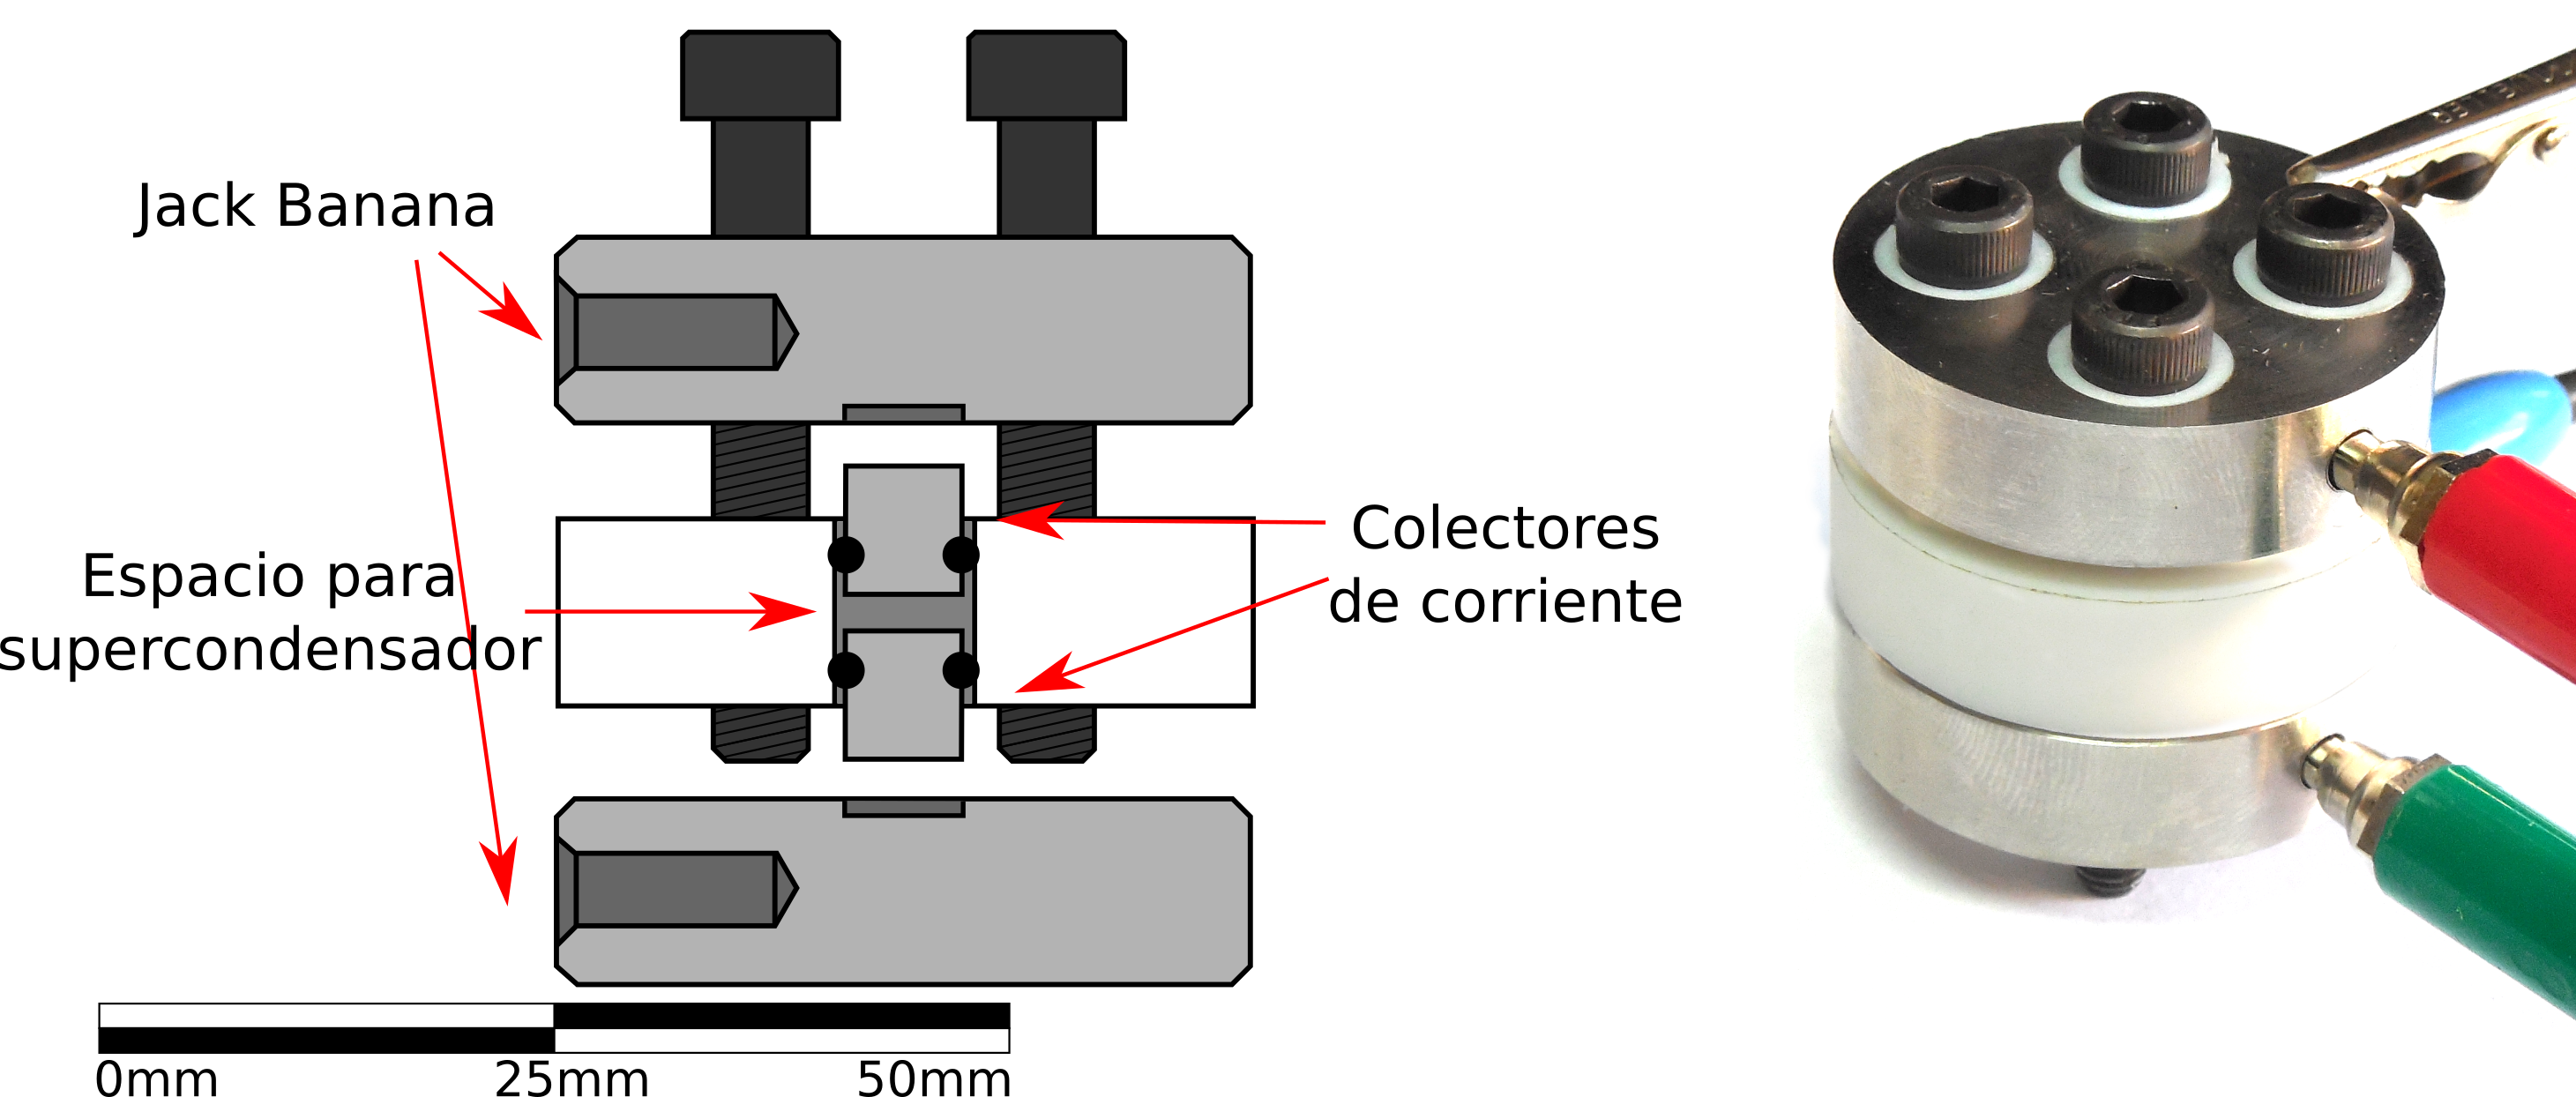
\includegraphics[width=0.8\textwidth]{cell3.png}
		}
	\caption{Izquierda: Vista longitudinal de la celda de pruebas, mostrando los componentes más importantes. Derecha: Fotografía de la celda armada y conectada al potenciostato.}
	\label{fig:celda_de_pruebas_SC}
\end{figure}

\section{Construcción de electrodos y preparación de electrolitos}
Los electrodos de rGO son fabricados mediante filtración por vacío. En este método de filtración, se dispersa el rGO en agua, la que se filtra por un filtro de celulosa en un embudo Büchner conectado a un kitasato y una bomba de vacío, el filtro con el material atrapado se deja secar a temperatura ambiente formando una lámina, la que es desprendida con facilidad del filtro de celulosa y luego recortada al tamaño apropiado para la celda de pruebas.

\begin{figure}
	\centering
	\fbox{
		\includegraphics[width=1.0\textwidth]{rgo_electrodes.png}
		}
	\caption{Electrodos utilizados en la celda de pruebas de supercondensador. De izquierda a derecha: Electro sin material depositado. Electrodo con material depositado mediante goteo (\emph{drop-casting}). Electrodo con material en forma de papel descentrado. Electrodo con material en forma de papel bien centrado soble el metal.}
	\label{fig:electrodes}
\end{figure}

\section{Resultados}
Los supercondensadores son sometidos a pruebas electroquímicas para estudiar su desempeño, estás pruebas incluyen: voltametría cíclica (CV), ciclos de carga y descarga a corriente constante, espectroscopía de impedancia electroquímica (EIS). Todas las mediciones electroquímicas son hechas con un potenciostato/galvanostato (Interface 5000E, Gamry).
